\let\negmedspace\undefined
\let\negthickspace\undefined
\documentclass[journal]{IEEEtran}
\usepackage[a5paper, margin=10mm, onecolumn]{geometry}
%\usepackage{lmodern} % Ensure lmodern is loaded for pdflatex
\usepackage{tfrupee} % Include tfrupee package

\setlength{\headheight}{1cm} % Set the height of the header box
\setlength{\headsep}{0mm}     % Set the distance between the header box and the top of the text

\usepackage{gvv-book}
\usepackage{gvv}
\usepackage{cite}
\usepackage{amsmath,amssymb,amsfonts,amsthm}
\usepackage{algorithmic}
\usepackage{graphicx}
\usepackage{textcomp}
\usepackage{xcolor}
\usepackage{txfonts}
\usepackage{listings}
\usepackage{enumitem}
\usepackage{mathtools}
\usepackage{gensymb}
\usepackage{comment}
\usepackage[breaklinks=true]{hyperref}
\usepackage{tkz-euclide} 
\usepackage{listings}
% \usepackage{gvv}                                        
\def\inputGnumericTable{}                                 
\usepackage[latin1]{inputenc}                                
\usepackage{color}                                            
\usepackage{array}                                            
\usepackage{longtable}                                       
\usepackage{calc}                                             
\usepackage{multirow}                                         
\usepackage{hhline}                                           
\usepackage{ifthen}                                           
\usepackage{lscape}
\begin{document}

\bibliographystyle{IEEEtran}
\vspace{3cm}

\title{4.11.6}
\author{EE25btech11028 - J.Navya sri}
% \maketitle
% \newpage
% \bigskip
{\let\newpage\relax\maketitle}

\textbf{Question:} \\
   Find the equation of the plane passing through the intersection of the planes 
\[
\mathbf{r}\cdot (\hat{i} + \hat{j} + \hat{k}) = 1
\]
and 
\[
\mathbf{r} \cdot (2\hat{i} + 3\hat{j} - \hat{k}) + 4 = 0
\]
and parallel to the $X$-axis. Hence, find the distance of the plane from the $X$-axis.
 
\bigskip
\textbf{Solution:}

\subsection*{Step1:Plane through Intersection}
Let the equations of the given planes be:
\begin{align}
\mathbf{r}  \cdot (\hat{i} + \hat{j} + \hat{k}) &= 1 \label{eq:plane1} \\
\mathbf{r} \cdot (2\hat{i} + 3\hat{j} - \hat{k}) &= 4 \label{eq:plane2}
\end{align}

Any plane passing through their intersection can be written as:
\begin{equation}
\left( \mathbf{r}  \cdot (\hat{i} + \hat{j} + \hat{k}) - 1\right) + \lambda \left(\mathbf{r}  \cdot (2\hat{i} + 3\hat{j} - \hat{k}) - 4 \right) = 0
\label{eq:intersect_plane}
\end{equation}

Expanding:
\begin{equation}
\mathbf{r}  \cdot \left( (\hat{i} + \hat{j} + \hat{k}) + \lambda (2\hat{i} + 3\hat{j} - \hat{k}) \right) = 1 + 4\lambda
\label{eq:expanded}
\end{equation}

The normal vector of the plane is:
\begin{equation}
\mathbf{N} = (1 + 2\lambda)\hat{i} + (1 + 3\lambda)\hat{j} + (1 - \lambda) \hat{k}
\label{eq:normal}
\end{equation}

\subsection*{Step2:Parallel to X-Axis}

Since the plane is parallel to the X-axis, its normal $\mathbf{N}$ must be perpendicular to the X-axis direction $\hat{i}$:
\begin{equation}
( \text{Coefficient of } \hat{i} \text{ in } \mathbf{N} ) = 0 \quad \implies \quad 1 + 2\lambda = 0 \implies \lambda = -\frac{1}{2}
\label{eq:lambda}
\end{equation}

Substitute $\lambda = -\frac{1}{2}$:
\begin{equation}
\mathbf{N}= 0 \cdot \hat{i} + \left(1 + 3\left(-\frac{1}{2}\right)\right)\hat{j} + \left(1 - \left(-\frac{1}{2}\right)\right)\hat{k} 
= -\frac{1}{2}\hat{j} + \frac{3}{2}\hat{k}
\label{eq:normal_final}
\end{equation}

Equation of the plane (using the scalar form $\mathbf{r} \cdot \mathbf{N} = D$):
\begin{align}
\mathbf{r}  \cdot \left(-\frac{1}{2}\hat{j} + \frac{3}{2}\hat{k}\right) &= 1 + 4\left(-\frac{1}{2}\right) = -1 \\
-\frac{1}{2}y + \frac{3}{2}z &= -1 \label{eq:plane_eq1} \\
-\frac{1}{2}y + \frac{3}{2}z + 1 &= 0 \quad \Rightarrow \quad -y + 3z + 2 = 0 \label{eq:plane_eq2}
\end{align}

\subsection*{Step3:Distance from X-Axis}

The X-axis is the line $y=0, z=0$.\\
Distance from the plane to the X-axis (taking point $(0,0,0)$) is:
\begin{equation}
D = \frac{| -0 + 3 \cdot 0 + 2 |}{\sqrt{(-1)^2 + 3^2}} = \frac{2}{\sqrt{10}}
\label{eq:distance}
\end{equation}

\subsection*{Final Answers:}

\begin{itemize}
    \item Required plane: $-y + 3z + 2 = 0$ 
    \item Distance from X-axis: $\dfrac{2}{\sqrt{10}}$
\end{itemize}



\textbf{Graph presentation:}
\begin{figure}[H]
\begin{center}
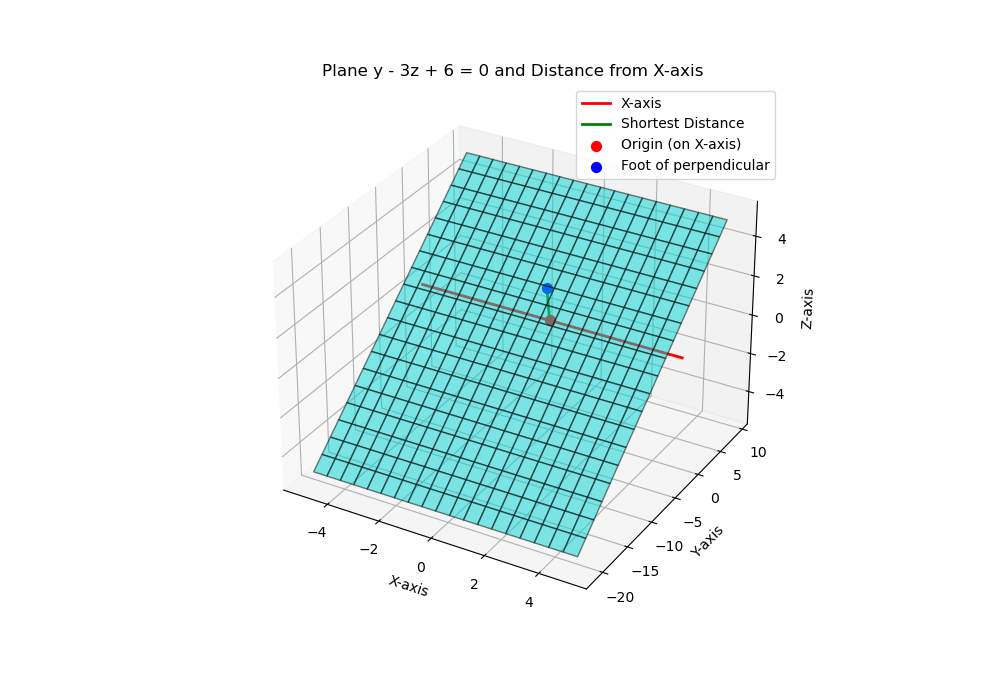
\includegraphics[width=0.6\columnwidth]{figs/fig8.png}
\end{center}
\caption{}
\label{fig:Fig}
\end{figure}
\end{document}
